% +---------------------------------------------------------------+
% | Author :    Noémie Plancherel, HEIG-VD
% | Date :      04.10.2022
% +---------------------------------------------------------------+

\chapter{Analyse de menaces}
\label{ch:analyse_menaces}

Ce chapitre a pour but d'identifier et analyser toutes les menaces existantes et / ou potentielles des \textit{password managers} en les modélisant en suivant un certain processus afin d'avoir une meilleure vision des risques.

Puis, nous allons rédiger toutes les exigences sécuritaires que doivent respecter les gestionnaires de mots de passe afin que ces dernières garantissent une utilisation sûre qui évite des pertes ou vol de données.

\section{Modélisation de menaces}
Afin de modéliser correctement les menaces, nous allons suivre la norme ISO 27005\cite{ISO27005}. Cela va nous permettre de séparer la modélisation en un processus avec plusieurs étapes comme suit:

\begin{enumerate}
	\item Établissement du contexte, qui inclut
	\begin{itemize}
		\item Objectifs des gestionnaires de mots de passe
		\item Hypothèses et exigences de sécurité
		\item Actifs à haute valeur 
		\item Data Flow Diagram
		\item Définition des critères d'analyse
	\end{itemize}
	\item Identification des risques
		\begin{itemize}
		\item Identification des biens
		\item Identification des menaces
		\item Identification des contrôles
		\item Identification des vulnérabilités
		\item Identification des conséquences
	\end{itemize}
	\item Analyse des risques
	\item Évaluation des risques
	\item Traitement des risques
	\item Documentation 
\end{enumerate}
La dernière étape ne sera pas explicitement abordée car elle vise à documenter le modèle de menaces que nous allons établir.

Pour chaque étape du processus, nous allons aborder les 3 types de gestionnaires existants; cloud-based, browser-based et local-based. On peut cependant les grouper en deux catégories différentes car le cloud-based et browser-based fonctionnent de la même manière lors de synchronisations de données.

Nous allons également nous baser sur le processus de modélisation de menaces de OWASP\cite{owasp}.
\subsection{Établissement du contexte}
Dans cette section, nous allons comprendre les applications et comment interagissent les gestionnaires de mots de passe avec les entités externes. Au final, nous allons établir un \textit{Data Flow Diagram} (DFD) qui va nous permettre de présenter tous les chemins différents du système en mettant en avant les vulnérabilités potentielles.

Comme cité plusieurs fois, l'objectif principal d'un gestionnaire de mots de passe est de stocker de manière \textbf{sûre} des informations sensibles, le plus souvent des identifiants, mais également la possibilité de stocker des notes, des informations bancaires, contrats, etc. Ils offrent également la fonctionnalité de générer des mots de passe fort et d'auto-compléter les champs de connexion.

On peut émettre plusieurs hypothèses de sécurité afin de mettre en avant ce que doit assurer le gestionnaire de mots de passe pour être considéré comme sûr. Nous séparons ces hypothèses en deux groupes; un concernant l'utilisateur et un concernant l'application en elle-même. 

\textbf{Utilisateur}
\begin{itemize}
	\item Master password fort
	\item Master password unique et différent d'autres identifiants de l'utilisateur
\end{itemize}

\textbf{Système}
\begin{itemize}
	\item Données du gestionnaire chiffrées / protégées
	\item Clés ou master password protégés dans la mémoire du processus ou complète
	\item Presse-papier effacé après un certain temps
	\item Utilisation d'algorithmes cryptographiques forts et recommandés
	\item Génération de mots de passe suffisamment forts
	\item Authentification des données
	\item Données effacées du disque lorsque le gestionnaire est dans un état \textit{Not Running} ou \textit{Locked}
	\item Base de données en local protégée
	\item Base de données des clés protégée (browser)
	\item Communication avec les serveurs chiffrée (cloud)
	\item Informations sensibles non-transmises en clair aux serveurs (cloud)
	\item Serveurs de confiance (cloud)
\end{itemize}

Nous pouvons à présent définir les actifs (\textit{assets}) des gestionnaires de mots de passe, qui représentent les éléments qui ont de la valeur et qui demandent une importante protection. 

Tout d'abord, un actif à haute valeur est l'\textbf{application} du gestionnaire de mots de passe. Cette dernière peut être sous forme d'application desktop, extension de navigateur ou application mobile. Nous voulons garantir:
\begin{itemize}
	\item Disponibilité
	\item Intégrité
\end{itemize}

Ensuite, un autre bien important est \textbf{la base de données} qui contient tous les identifiants, notes, informations bancaires, stockées par l'utilisateur. Le bien principal sont donc les données. Nous pouvons également inclure le processus de chiffrement du coffre-fort comme bien principal. Nous souhaitons garantir les éléments suivants:
\begin{itemize}
	\item Confidentialité des données
	\item Intégrité des données
\end{itemize}


Un autre actif à haute valeur sont les \textbf{clés de chiffrement} (ou les clés privées dans le cadre de partage de données avec d'autres utilisateurs). Nous incluons également le processus de génération de clés. Nous voulons garantir ces éléments:
\begin{itemize}
	\item Confidentialité 
	\item Intégrité
\end{itemize}

Finalement, dans le cadre de gestionnaires de mots de passe cloud-based (ou browser-based) qui ne fonctionnent pas en mode offline, nous voulons protéger les données des \textbf{serveurs} du provider. Le processus de transfert de données est également important car les données doivent impérativement être protégées. Ainsi, nous souhaitons assurer:
\begin{itemize}
	\item Confidentialité
	\item Disponibilité du service
\end{itemize}

À présent, nous allons définir le DFD afin de correctement décomposer le système. Pour avoir la meilleure vue d'ensemble, nous allons faire un diagramme pour les gestionnaires local-based et un autre pour les cloud-based / browser-based.


\begin{figure}[H]
	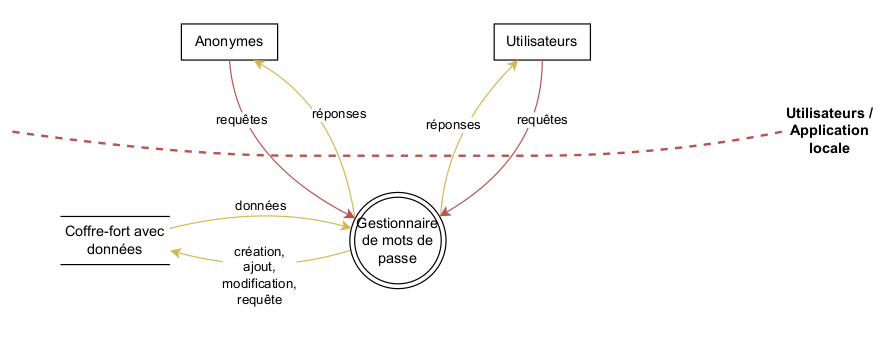
\includegraphics[width=15.5cm]{images/dfd_local.png}
	\centering
	\caption{Data Flow Diagram pour les gestionnaires local-based}
\end{figure}

\begin{figure}[H]
	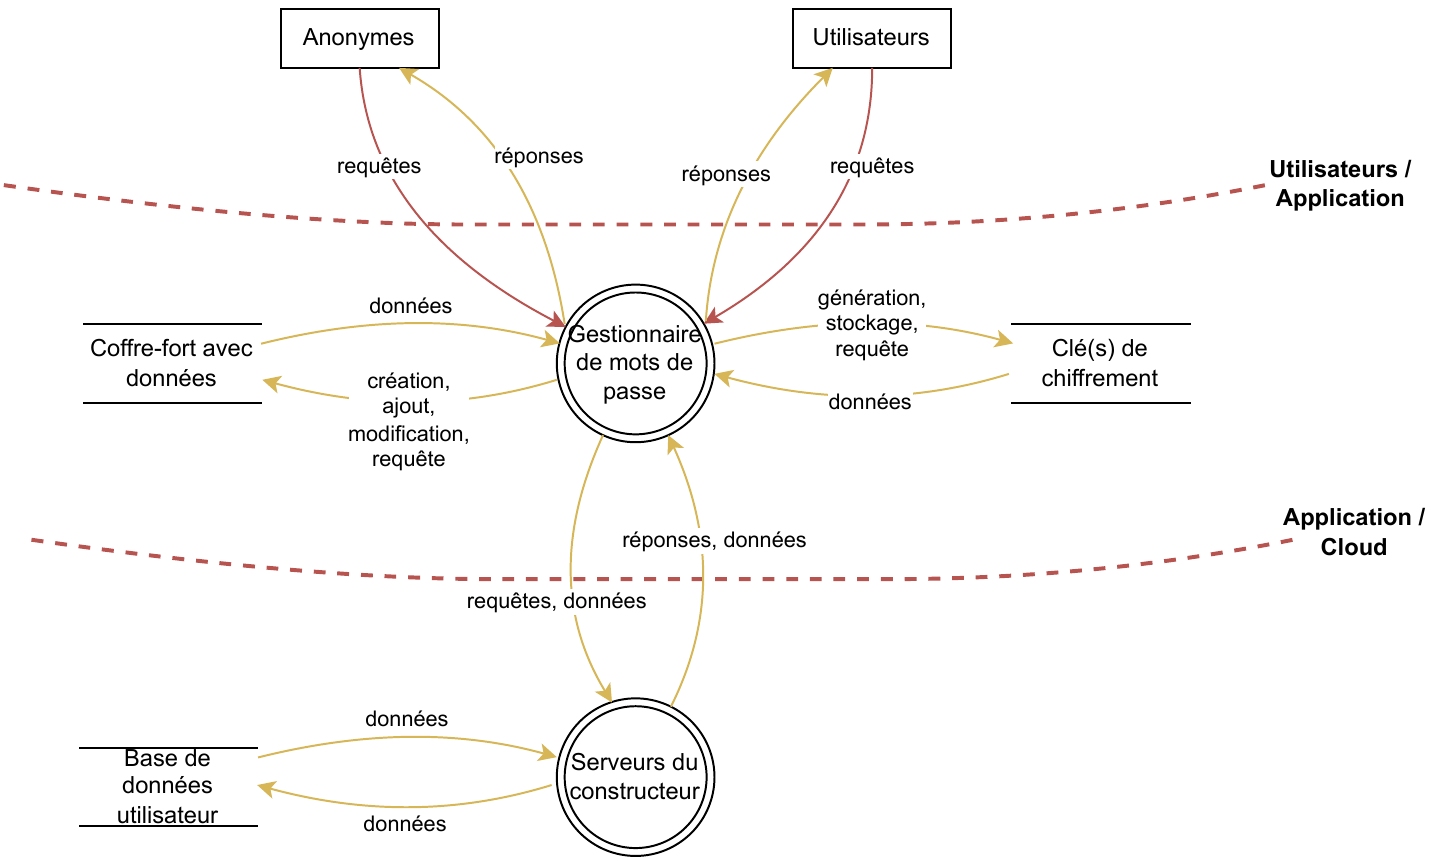
\includegraphics[width=15.5cm]{images/dfd_cloud.png}
	\centering
	\caption{Data Flow Diagram pour les gestionnaires cloud-based et browser-based}
\end{figure}

Dernièrement, nous allons définir les différents critères et niveaux pour évaluer l'impact des événements (les conséquences), la probabilité d'événement, la sévérité des vulnérabilités ainsi que l'évaluation des risques. Ces niveaux seront réutilisés pour l'identification des risques dans la suite de l'analyse de menaces.

\begin{table}[H]
	\begin{tabular}{llc}
		\hline
		Échelle  & Description                                                                                                                                                                                               & Valeur   \\ \hline
		Aucune   & La vulnérabilité ne présente aucune sévérité                                                                                                                                                              & 0        \\
		Bas      & \begin{tabular}[c]{@{}l@{}}La vulnérabilité a peu d'impact sur l'entreprise et demande un\\ accès physique ou local au système\end{tabular}                                                               & 0.1-39   \\
		Moyen    & \begin{tabular}[c]{@{}l@{}}En général, elle demande à l'attaquant d'être sur le même réseau \\ que la victime et elle demande les privilèges utilisateurs pour \\ effectuer une exploitation\end{tabular} & 4.0-6.9  \\
		Haut     & \begin{tabular}[c]{@{}l@{}}La vulnérabilité est difficile à exploter, peut être une élévation de \\ privilèges et peut amener à une importante perte de données ou \\ de temps d'arrêt\end{tabular}       & 7.0-8.9  \\
		Critique & \begin{tabular}[c]{@{}l@{}}Exploitation de vulnérabilités au niveau root, l'attaquant n'a pas\\ besoin d'être authentifié ou avoir des connaissances sur la victime\end{tabular}                          & 9.0-10.0 \\ \hline
	\end{tabular}
	\caption{Scores de sévérité basés sur CVSS v3.1}
\end{table}

\begin{table}[H]
	\centering
	\resizebox{\textwidth}{!}{\begin{tabular}{llc}
		\hline
		Échelle        & Description                                                                                                                                                                                                    & Valeur \\ \hline
		Négligeable    & L'impact sur l'entreprise est négligeable                                                                                                                                                                      & 0      \\
		Mineur         & \begin{tabular}[c]{@{}l@{}}L'effet sur les biens de l'entreprise est limité, comme entraîner des \\ pertes financières mineures ou entraîner des dommages mineures \\ aux actifs de l'entreprises\end{tabular} & 1      \\
		Modéré         & \begin{tabular}[c]{@{}l@{}}L'effet sur les biens peut être grave, les effets causés sur les biens \\ seront considérés comme importants\end{tabular}                                                           & 2      \\
		Important      & L'effet sur les biens de l'entreprise peut être grave à catastrophique                                                                                                                                         & 3      \\
		Catastrophique & \begin{tabular}[c]{@{}l@{}}On s'attend à ce que la menace ait de multiples effets graves à \\ catastrophiques sur les biens de l'entreprise\end{tabular}                                                       & 4      \\ \hline
	\end{tabular}}
\caption{Impact des menaces sur l'entreprise}
\end{table}

\begin{table}[H]
	\centering
	\begin{tabular}{llc}
		\hline
		Échelle      & Description                                            & Valeur \\ \hline
		Rare         & La probabilité que l'événement arrive est rare         & 0      \\
		Peu probable & La probabilité que l'événement arrive est peu probable & 1      \\
		Possible     & La probabilité que l'événement arrive est possible     & 2      \\
		Probable     & La probabilité que l'événement arrive est probable     & 3      \\
		Certain      & La probabilité que l'événement arrive est certain      & 4      \\ \hline
	\end{tabular}
\caption{Probabilités d'événements}
\end{table}

Pour l'évaluation des risques, il est important de prendre en considération la probabilité d'événements et les conséquences sur l'entreprise afin de définir une échelle d'évaluation de risques. Nous utilisons une matrice de risques basée sur une étude quantitative.

\begin{figure}[H]
	\centering
	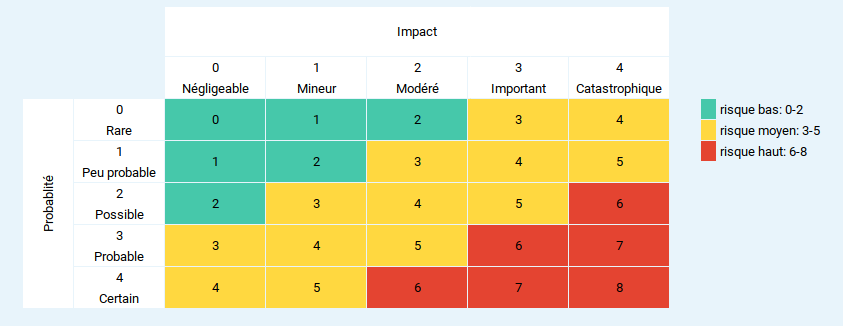
\includegraphics[width=15.5cm]{images/risque_evaluation.png}
	\centering
	\caption{Critères d'évaluation des risques \label{Critères d'évaluation des risques}}
\end{figure}

\subsection{Identification des risques}
Cette section va nous servir à déterminer ce qui peut se produire pour causer une perte potentielle et à comprendre comment, où et pourquoi la perte peut se produire. 

Afin d'établir une étude complète, nous allons premièrement identifier les biens, menaces (avec les sources de menaces et les scénarios), les contrôles, les vulnérabilités ainsi que les conséquences sur l'entreprise.

Dans chaque table, pour chaque élément cité, nous précisons les types de gestionnaires de mots de passe concernés; L (local-based), B (browser-based), C (cloud-based).

\textbf{Identification des biens}

Nous avons déjà identifié les actifs plus-haut dans l'analyse, cependant nous allons ajouter un code pour les identifier et les référencer plus tard dans l'identification des risques

\begin{table}[H]
	\centering
	\resizebox{\textwidth}{!}{\begin{tabular}{llll}
		\hline
		Code & Bien                                & Description                                                         & Type    \\ \hline
		A1   & Application & L'application du gestionnaire de mots de passe                      & L, B, C \\
		A2   & Base de données                     & Base de données avec toutes les informations stockées               & L, B, C \\
		A3   & Clés de chiffrement                 & Clés de chiffrement ou clés pour le partage de données              & L, B, C \\
		A4   & Serveurs du provider                & Serveurs dans le cloud où sont stockés les données de l'utilisateur & B, C    \\ \hline
	\end{tabular}}
\caption{Biens des gestionnaires de mots de passe}
\end{table}
\textbf{Identification des menaces}

Nous allons identifier toutes les sources de menaces possibles des gestionnaires de mots de passe avec leurs motivations (uniquement si c'est de source humaine) afin de pouvoir mettre en avant les différents scénarios de menaces.

\begin{table}[H]
	\centering
	\begin{tabular}{cll}
		\hline
		Code & Source de menace                & Motivations                               \\ \hline
		S1   & Hackers & Amusement, gloire, challenge, argent, ego \\
		S2   & Script kiddies                  & Curiosité, ego, argent, amusement         \\
		S3   & Concurrent                      & Espionnage, réutilisation de contenu      \\
		S4   & Cybercrime                      & Argent, destruction de données            \\
		S5   & Accident humain                 & -                                         \\
		S6   & Problèmes techniques            & -                                         \\ \hline
	\end{tabular}
\caption{Sources de menaces des gestionnaires de mots de passe}
\end{table}

Ci-dessous, se trouve un tableau avec différents scénarios de menaces par rapport aux biens que nous avons défini précédemment. Nous nous basons sur le modèle STRIDE afin de définir les types de menaces. 
\begin{table}[H]
		\centering
	\resizebox{\textwidth}{!}{\begin{tabular}{cccllll}
			\hline
			& Code & Code du bien & Scénario de menace                                                                                                            & Type de menace                & Source de menace & Type    \\ \hline
			1 & T1   & A1           & Brute-force sur le master password                                                                                            & \textit{Spoofing}      & S1, S2, S4, S5   & L, B, C \\
			2 & T2   & A1           & \begin{tabular}[c]{@{}l@{}}Key-logger installé sur le device de l'utilisateur \\ et qui sniff le master password\end{tabular} & \textit{Elevation of privileges}    & S1, S2, S4       & L, B, C \\
			3 & T2   & A1           & \begin{tabular}[c]{@{}l@{}}Utilisateur non-déconnecté de son compte \\et attaquant a accès au device\end{tabular}                                                                                     & \textit{Elevation of privileges}      & S1, S2, S4, S5   & L, B, C \\
			4 & T1   & A1           & Mauvais mécanisme d'authentification                                                                                          & \textit{Spoofing}    & S1, S2, S4, S6   & L, B, C \\
			5 &T3   & A1           & Lecture du presse-papier                                                                                                      & \textit{Information disclosure}    & S1, S2, S4       & L, B, C \\
			6 & T1   & A1           & Phishing en imitant une page de connexion                                                                                     & \textit{Spoofing}   & S1, S2, S3, S4   & B, C    \\
			7 & T1   & A1           & \begin{tabular}[c]{@{}l@{}}Attaque XSS avec les champs de connexion\\ auto-complétés\end{tabular}                             & \textit{Spoofing}     & S1, S2, S4       & B, C    \\
			8 & T1   & A1           & \begin{tabular}[c]{@{}l@{}}Coffre-fort compromis dû à des identifiants volés\\ sur d'autres sites\end{tabular}                & \textit{Spoofing}      & S1, S2, S4, S5   & L, B, C \\
			9 & T3   & A1           & Récupération de données sensibles en clair sur le disque                                                                      & \textit{Information disclosure}      & S1, S2, S4       & L, B, C \\
			10 & T3   & A1           & Clickjacking                                                                                                                            & \textit{Information Disclosure}           & S1, S2, S4   & B, C \\
			11 & T3   & A2           & \begin{tabular}[c]{@{}l@{}}Récupération de la base de données et déchiffrement\\ dû à un algorithme trop simple\end{tabular}  & \textit{Information disclosure}    & S1, S2, S4       & L, B, C \\
			12 & T3   & A2           & Récupération de données sensibles en mémoire                                                                                  & \textit{Information Disclosure}    & S1, S2, S4       & L, B, C \\
			13 & T6   & A2           & Injection SQL dans le base de données utilisateur                                                                                                                           & \textit{Tampering}           & S1, S2, S4   & L, B, C			\\
			14 & T3   & A3           & Récupération de la clé de chiffrement en mémoire                                                                              & \textit{Information Disclosure}    & S1, S2, S4       & L, B, C \\
			15 & T3   & A3           & Brute-force de clé                                                                                                            & \textit{}    & S1, S2, S4       & L, B, C \\
			16 & T3   & A4           & MITM (Interception de données non-chiffrées)                                                                                  & \textit{Information Disclosure}          & S1, S2, S4, S6   & B, C    \\
			17 & T3   & A4           & Vols de données non protégées sur le serveur                                                                                  & \textit{Information disclosure} & S1, S2, S4, S6   &         \\
			18 & T4   & A4           & DoS                                                                                                                           & \textit{Denial of service}           & S1, S2, S4, S6   & B, C   		\\
			19 & T5   & A4           & Perte des données utilisateurs dû à un serveur down                                                                                                                           & \textit{Equipment failure}           & S5, S6   & B, C   	\\
			\\\\	\hline 
			\multicolumn{7}{l}{A1 = Application | A2 = Base de données | A3 = Clés | A4 = Serveurs du provider}\\ \hline
	\end{tabular}}
\caption{Scénarios et types de menaces possibles \label{4.3}}
\end{table}

\textbf{Identification des contrôles}\label{contrôles}

Une étape important lors de l'identification des risques et d'identifier les contrôles qui existent déjà sur les applications sur lesquelles nous basons notre analyse de risques. Étant donné, que notre étude est plutôt générale car elle ne se base pas sur un seul gestionnaires de mots de passe, nous allons énumérer les contrôles qui ont été entrepris afin de baisser le niveau de risque. Nous parlerons en détails des contrôles effectués lors de la seconde partie du travail.

Le contrôle qui est présent sur toutes les applications est que chaque utilisateur possède une clé de chiffrement différente, qui est dérivée avec son master password. Même si ce dernier est le même, la clé ne sera pas pareille dû au salt qui est soit aléatoire soit le username, qui est unique. Les algorithmes choisis sont forts (voir \ref{crypto}) et sont recommandés pour la dérivation des clés. Ainsi, la clé est protégée contre le brute-force ou les attaques par dictionnaire. Néanmoins, il est quand même important d'avoir un master password fort\footnote{Ce qu'on considère un mot de passe fort; au moins une majuscule, une minuscule, un chiffre et 8 caractères}, ce qui n'est pas demandé dans tous les gestionnaires de mots de passe lors de l'inscription de l'utilisateur.

Au niveau du chiffrement des données, les gestionnaires local-based et cloud-based, utilisent AES-256. L'algorithme est également encore recommandé en 2022.

Au niveau de la protection mémoire, certains proposent une protection des données sensibles dans le processus (avec DPAPI ou Chacha20) et les données sont effacées sur le disque dès que le processus s'arrête. En se basant sur une étude\cite{iseexploit}, la mémoire est en général bien protégée lorsque le gestionnaire dans l'état \textit{not running}, cependant dès le moment où le gestionnaire est dans l'état \textit{unlock} ou \textit{locked}, les secrets et le master password sont plus exposés. 

Au niveau de la protection du keylogger, aucune protection n'est réellement implémentée, à part utiliser l'application dans environnement sécurisé comme \textit{Secure Desktop} sur Windows. Pour la protection du presse-papier, certaines applications (comme 1Password ou Keepass) mettent à disposition une fonctionnalité pour enlever les données sensibles du presse-papier après un certain moment.

Finalement, pour l'auto-complétion des champs de connexion, certains s'assurent que l'utilisateur valide s'il veut vraiment remplir ce champ afin d'éviter d'entrer les données sensibles dans des pages web clonées malveillantes.

\textbf{Identification des vulnérabilités}

Pour chaque actif identifié au préalable, nous allons analyser les vulnérabilités qui pourraient être présentes. Nous allons également ajouter la sévérité de la vulnérabilité. 

\begin{table}[H]
	\centering
	\resizebox{\textwidth}{!}{\begin{tabular}{clll}
				\hline
				Bien                   & Vulnérabilité                                                                                                          & Sévérité de la vulnérabilité & Type    \\ \hline
				A1                     & Master password trop faible                                                                                            & Haut                         & L, B, C \\
				A1                     & Temps de session long                                                                                                  & Critique                     & L, C    \\
				A1                     & Presse-papier non nettoyé après un certain temps                                                                       & Moyen                        & L, B, C \\
				A1                     & Master password non unique                                                                                             & Bas                          & L, B, C \\
				A1                     & 2FA pas proposé par défaut                                                                                             & Haut                         & L, B, C \\
				A1                     & Aucune protection de la mémoire du processus                                                                           & Haut                         & L, B, C \\
				A1                     & Aucune authentification effectuée                                                                                      & Moyen                        & L, B, C \\
				A1                     & Option \textit{remember me}                                                                                                   & Haut                         & L, C    \\
				A1                     & Génération de mots de passe faibles                                                                                    & Haut                         & L, B, C \\
				A1                     & \begin{tabular}[c]{@{}l@{}}Auto-complétion de champs sans une\\ interaction avec l'utilisateur\end{tabular}            & Moyen                        & B, C    \\
				A1                     & \begin{tabular}[c]{@{}l@{}}Utilisation de critères de correspondance \\ faibles lors de l'auto-complétion\end{tabular} & Moyen                        & B, C    \\
				\multicolumn{1}{c}{A1} & \begin{tabular}[c]{@{}l@{}}Données non nettoyées sur le disque lors de \\ l'arrêt du processus\end{tabular}            & Haut                         & L, B, C \\
				A1                     & Manque de contrôle des entrées utilisateurs                                                                                                   & Haut                         & L, B, C    \\
				A1                     & \begin{tabular}[c]{@{}l@{}}Règles d'auto-complétion HTTP ne différencie \\ pas HTTP et HTTPS\end{tabular}                                                                                                             & Haut                         & B, C    \\				
				A2, A3                 & \begin{tabular}[c]{@{}l@{}}Utilisation d'algorithmes de chiffrement plus \\ recommandés ou trop faibles\end{tabular}   & Haut                         & L, B, C \\
				A2, A4                 & Informations stockées en clair                                                                                         & Haut                         & L, B, C \\
				A3                     & Dérivation des clés trop simple                                                                                        & Moyen                        & L, C    \\
				A4                     & Communication non-chiffrée                                                                                             & Critique                     & B, C    \\
				A4                     & Backup non effectué                                                                                                    & Critique                     & B, C   
				\\ \\ \hline
					\multicolumn{4}{l}{A1 = Application | A2 = Base de données | A3 = Clés | A4 = Serveurs du provider}\\ \hline
			\end{tabular}}
	\caption{Vulnérabilités présentes dans les gestionnaires de mots de passe}
\end{table}

\textbf{Identifications des conséquences}

Il est également important d'identifier les conséquences qui pourraient être causés par un incident. Nous allons définir par bien actif quelles sont les conséquences qu'ils pourraient y avoir sur l'entreprise lors d'une perte de confidentialité, intégrité ou disponibilité. Pour cela, nous allons nous référer au tableau \ref{4.3} qui définit différents scénarios de menaces. 

\begin{table}[H]
	\centering
	\begin{tabular}{ll}
		\hline
		Bien                     & Conséquences                                                                                                     \\ \hline
		Application (A1)         & Perte de réputation et d'image                                                                                 \\
		Base de données (A2)     & Perte de réputation et d'image, perte de données                     \\
		Clés de chiffrement (A3) & Perte de réputation et d'image, perte de données                \\
		Serveurs (A4)            & \begin{tabular}[c]{@{}l@{}}Perte de réputation et d'image, coûts financiers, \\coûts de réparation\end{tabular} \\ \hline
	\end{tabular}
\caption{Conséquences des menaces sur l'entreprise}
\end{table}

\subsection{Analyse des risques}
L'objectif de cette section est d'estimer la probabilité des incidents et les conséquences pour les biens qu'ils menacent. Pour ce faire, nous allons faire une analyse de risque qualitative ce qui va nous permettre de faire une première analyse de risques assez générale afin de nous permettre d'aller plus en détails dans la seconde partie du travail de Bachelor.

Ainsi, nous allons analyser l'impact des conséquences ainsi que la probabilité que chaque scénario d'attaque identifié puisse se produire. Pour cela, nous allons utiliser plusieurs notations différentes; pour les conséquences nous aurons les niveaux suivants:

	\begin{table}[H]
		\centering
		\resizebox{\textwidth}{!}{\begin{tabular}{cclllll}
				\hline 
		Bien & Menace & Scénario                                                                                                                     & Impact des conséquences & Probabilité  & Niveau de risque \\ \hline
		A1   & T1     & Brute-force sur le master password                                                                                           & Important               & Certain      & Haut            \\
		A1   & T2     & \begin{tabular}[c]{@{}l@{}}Key-logger installé sur le device de l'utilisateur\\ et qui sniff le master password\end{tabular} & Important               & Possible     & Moyen            \\
		A1   & T2     & \begin{tabular}[c]{@{}l@{}}Utilisateur non-déconnecté de son compte\\ et attaquant a accès au device\end{tabular}            & Important               & Probable     & Haut             \\
		A1   & T1     & Mauvais mécanisme d'authentification                                                                                         & Modéré                  & Rare         & Bas            \\
		A1   & T3     & Lecture du presse-papier                                                                                                     & Modéré                  & Probable     & Moyen            \\
		A1   & T1     & Phishing en imitant une page de connexion                                                                                    & Modéré                  & Possible     & Moyen            \\
		A1   & T1     & \begin{tabular}[c]{@{}l@{}}Attaque XSS avec les champs de connexion\\ auto-complétés\end{tabular}                            & Important               & Possible     & Moyen            \\
		A1   & T1     & \begin{tabular}[c]{@{}l@{}}Coffre-fort compromis dû à des identifiants \\ volés sur d'autres sites\end{tabular}              & Mineur                  & Possible     & Moyen              \\
		A1   & T3     & Clickjacking                                                                     & Modéré          & Possible     & Moyen             \\
		A1   & T3     & Récupération de données sensibles en clair sur le disque                                                                     & Important          & Probable     & Haut             \\
		A2   & T3     & \begin{tabular}[c]{@{}l@{}}Récupération de la base de données et déchiffrement\\ dû à un algorithme trop simple\end{tabular} & Important          & Peu probable & Moyen            \\
		A2   & T3     & Récupération de données sensibles en mémoire                                                                                 & Important          & Probable     & Haut             \\
		A2   & T6     & Injection SQL dans la base de données                                                                                 & Important          & Peu probable     & Moyen             \\
		A3   & T3     & Récupération de la clé de chiffrement en mémoire                                                                             & Important          & Probable     & Haut             \\
		A3   & T3     & Brute-force de clé                                                                                                           & Important               & Peu probable & Moyen              \\
		A4   & T3     & MITM (Interception de données non-chiffrées)                                                                                 & Catastrophique               & Peu probable & Moyen              \\
		A4   & T3     & Vols de données non protégées sur le serveur                                                                                 & Important               & Rare         & Moyen              \\
		A4   & T4     & DoS                                                                                                                          & Modéré                  & Possible     & Moyen              \\
		A4   & T5     & Perte des données utilisateurs dû à un serveur down                                                                          & Catastrophique           & Peu probable & Moyen            \\ \\\hline 
			\multicolumn{6}{l}{A1 = Application | A2 = Base de données | A3 = Clés | A4 = Serveurs du provider}\\ 
				\multicolumn{6}{l}{T1 = Spoofing | T2 = Elevation of privileges | T3 = Information Disclosure | T4 = Denial of service | T5 = Equipment failure | T6 = Tampering}\\ 
			\hline
	\end{tabular}}
\caption{Analyse des risques de chaque scénario de menace}
\end{table}

\subsection{Évaluation des risques}

Cette étape sert à évaluer si les risques sont acceptables ou s'ils ont besoin d'un traitement supplémentaires, c'est-à-dire une mitigation. Nous avons défini à l'étape précédente le niveau de risque de chaque scénario de menace. En résumé, nous avons:

\begin{itemize}
	\item Bas: 1
	\item Moyen: 13
	\item Haut: 5
\end{itemize} 

Ainsi, nous pouvons définir que les tous les scénarios de menaces ayant un niveau de risque bas peuvent être acceptés par l'entreprise, néanmoins ces derniers ne doivent pas être oubliés et mis de côté. Pour les niveaux de risques moyen et haut, il est nécessaire d'appliquer une mitigation et de surveiller les menaces. 

\subsection{Traitement des risques}
Dans cette section, nous allons définir les contre-mesures à entreprendre afin d'éviter au maximum les menaces que nous avons identifié plus haut. Comme précisé dans le paragraphe de l'identification des contrôles \ref{contrôles}, beaucoup de choses sont déjà mises en place par les constructeurs et sont efficaces contre les attaques. Néanmoins, nous pouvons ajouter quelques contre-mesures qui ne sont pas ou peu effectuées par les quelques candidats que nous avons sélectionnés au préalable. Ainsi, nous allons sélectionner les risques qui ont été qualifiés comme moyen ou haut et nous allons proposer des contre-mesures possibles.

	\begin{table}[H]
	\centering
	\resizebox{\textwidth}{!}{\begin{tabular}{l|l}
		\hline
		Menace                                    & Contre-mesures                                                                                                                                                                                                                                                                                                           \\ \hline
		Master password faible                    & \begin{tabular}[c]{@{}l@{}}- Ajouter des contrôles lors de l'inscription de l'utilisateur en lui demandant un mot de passe fort\\ - Proposer un master password fort généré aléatoirement par l'application\end{tabular}                                                                                                 \\ \hline
		Temps de session trop long                & - Ajouter un temps d'expiration de session et verrouiller le gestionnaire après ce temps                                                                                                                                                                                                                                 \\ \hline
		Presse-papier non nettoyé                 & - Après un temps court, nettoyer le presse-papier de l'utilisateur                                                                                                                                                                                                                                                       \\ \hline
		Phishing en clonant une page de connexion & \begin{tabular}[c]{@{}l@{}}- Appliquer un meilleur critère de match lors de l'auto-complétion des champs\\ de connexion\\ - Demander à l'utilisateur de valider l'auto-complétion\end{tabular}                                                                                                                           \\ \hline
		Clickjacking                              & - Bloquer l'utilisation de Javascript à l'aide d'API sécurisées                                                                                                                                                                                                                                                          \\ \hline
		Communication non-chiffrée                & \begin{tabular}[c]{@{}l@{}}- Ajouter HTTPS pour la communication avec le serveur\\ - Éviter d'envoyer le master password ou des clés de chiffrement ou\\ privée au serveur\\ - Chiffrer toutes les données avant de les envoyer dans le cloud\end{tabular}                                                               \\ \hline
		Dérivation des clés trop simple           & \begin{tabular}[c]{@{}l@{}}- Utiliser un algorithme recommandé et fort (PBKDF2-SHA2 par exemple)\\ - Une clé de chiffrement unique par utilisateur pour éviter le brute force\end{tabular}                                                                                                                               \\ \hline
		Perte de données                          & \begin{tabular}[c]{@{}l@{}}- Si cloud-based / browser-based, effectuer des backups sur les serveurs chaque\\ nuit\\ - Mettre à disposition la fonctionnalité de backup pour les particuliers pour les \\ faire en local\\ - Exportation des données CSV et les stocker dans un endroit chiffrer et sécurisé\end{tabular} \\ \hline
		Manque de protection dans la mémoire      & \begin{tabular}[c]{@{}l@{}}- Nettoyage de mémoire lorsque le gestionnaire est dans l'état locked\\ - Protection des données sensible avec des APIs pour limiter l'exposition\\ de secrets\end{tabular}                                                                                                                   \\ \hline
		\multicolumn{1}{l|}{Option remember me}  & \multicolumn{1}{l}{- Désactivation de mode offline avec les gestionnaires cloud-based et browser-based}                                                                                                                                                                                                                 \\ \hline
	\end{tabular}}
\caption{Contre-mesures possibles pour les gestionnaires}
\end{table}

\section{Exigences sécuritaires à respecter} 
Dans cette dernière section de l'analyse de menaces, nous allons établir une liste d'exigences sécuritaires que les gestionnaires de mots de passe doivent respecter afin de se définir sécurisé et afin de protéger les données sensibles au maximum. Pour cela, nous allons lister les exigences générales ainsi que les exigences par type d'applications (cloud, browser et local).

\textbf{Chiffrement des données}

Le chiffrement du coffre-fort qui contient toutes les données personnelles et sensibles de l'utilisateur doit impérativement être chiffré avec un algorithme ainsi qu'une taille de clé qui sont recommandés. Nous pouvons nous baser sur les recommandations du report de ECRYPT\cite{ecrypt}. Au mieux, l'algorithme devrait être encore recommandé pour une utilisation future.

Pour les gestionnaires cloud-based et browser-based, dès le moment où il y a une interaction avec les serveurs du constructeur, le chiffrement devrait être \textit{end-to-end} pour assurer la protection des données lors du transport dans le cloud.

\textbf{Clés de chiffrement}

L'algorithme utilisé pour la génération de clé.s en dérivant le mot de passe devrait se baser sur des algorithmes \textit{Password-Based Key Derivation} et s'assurer qu'il fasse partie des recommandations d'ECRYPT. Les plus couramment utilisés sont Argon2 ou PBKDF2 (associé à une fonction de hash). Pour le salt, il doit absolument être unique. Le mieux serait d'utiliser un pseudo-nombre généré aléatoirement (PRNG) afin de s'assurer que ce nombre soit correctement aléatoire. Ce dernier devrait être stocké de manière sûre en local chez l'utilisateur. Une autre manière de faire, plus simple pour la gestion du salt aléatoire, est de prendre le username de l'utilisateur, qui peut être soit une adresse e-mail soit le nom d'utilisateur. Cependant, lors de l'inscription, il faut absolument que ce dernier soit unique afin d'éviter que des coffre-forts puissent avoir la même clé.

Pour le cloud-based et browser-based, la clé ne doit jamais être envoyée aux serveurs et doit rester en local dans la mémoire du processus. 

\textbf{Authentification des données et de l'utilisateur}

Pour les gestionnaires local-based / offline, étant donné qu'il n'y a aucune interaction avec un serveur externe, il est nécessaire d'authentifier les données afin d'assurer l'intégrité et la confidentialité. Il est bien d'utiliser un schéma \textit{Encrypt-then-MAC} qui est le chiffrement authentifié le plus sûr. 

Pour les gestionnaires cloud-based ou browser-based, il est nécessaire d'authentifier les utilisateurs auprès des serveurs du constructeur. Pour cela, il existe plusieurs manières de faire et nous allons pas aller en détails dans cette section, mais le hash d'authentification doit être envoyé aux serveurs de manière sécurisée, c'est-à-dire que la communication doit être chiffrée avec HTTPS. Le hash d'authentification à être comparé avec celui envoyé par l'utilisateur, doit être stocké dans la base de données de l'utilisateur sur les serveurs, chiffré pour garder sa confidentialité. 

\textbf{Master password}

Au mieux, il serait un bon réflexe, d'ajouter des exigences sécuritaires au niveau du master password lors de l'inscription de l'utilisateur. Ainsi, on peut s'assurer que le master password est fort et on peut éviter au maximum les attaques de brute-force ou par dictionnaires.

Le master password ne devrait jamais être stocké en mémoire afin d'éviter tout vol. Ainsi, la fonctionnalité de se souvenir du master password est fortement à déconseiller, à moins que des précautions de protection de mémoire aient été prises. 

Une bonne pratique serait d'activer le 2FA ou MFA obligatoire par défaut afin d'ajouter une couche sécuritaire. 

Pour les applications cloud-based ou browser-based, les serveurs ne devraient pas avoir connaissance du master password et il ne devrait jamais être transmis. 

\textbf{Session}

Pour éviter que si une personne malveillante puisse accéder à votre device et exploite le gestionnaire de mots de passe, il est nécessaire d'ajouter un temps de session. Après ce court temps, l'application devrait se mettre dans un état \textit{Locked} pour déconnecter l'utilisateur du coffre-fort.

\textbf{Mémoire}

Comme on l'a expliqué précédemment (\ref{etats}), chaque état différent de la mémoire doit absolument garantir différents éléments. Dans l'état \textit{Not Running}, aucune donnée sensible ne doit rester sur le disque; tout doit être nettoyé lors de l'arrêt du processus. Dans l'état \textit{Unlocked State}, on doit garantir qu'il n'est pas possible d'extraire de données sensibles en mémoire (en faisant un dump de mémoire par exemple). Finalement, dans l'état \textit{Locked}, toutes les données doivent être effacées du disque pour éviter quelconque extraction. 

\textbf{Presse-papier}

Il est très important d'éviter des attaques de sniffing de presse-papier, pour cela, il est nécessaire de nettoyer ce dernier après un court instant (10-40 secondes) et également s'assurer que l'historique du presse-papier est effacé.

\textbf{Phishing (et autres attaques web-based) et auto-complétion}

Finalement, les dernières exigences qu'on peut lister sont en rapport aux attaques Web; phishing, clickjacking, XSS, etc. Premièrement dans le cadre d'auto-complétion dans les formulaires de login, il est nécessaire demander à l'utilisateur de valider le remplissage que propose le gestionnaire pour s'assurer qu'il n'y a aucun risque. 

Puis, on peut également redéfinir les critères de matching pour les URLs afin de s'assurer qu'ils soient stricts. Un autre point important où il faut assurer une protection est pour le sous-domaine de l'URL, quelques gestionnaires ignorent le sous-domaine, ainsi il serait possible de voler les identifiants du domaine parent. 

Il est nécessaire faire une différence avec HTTP et HTTPS lors du remplissage de formulaire afin de ne pas subir une attaque MITM et de remplir une page clonée HTTP d'un site initialement en HTTPS. 

Finalement, il faudrait bloquer l'exécution Javascript dans le cadre de gestionnaires cloud-based ou browser-based afin d'éviter toute exécution de code malveillant et non-souhaité.
